	\def\year{2017}\relax
	%File: formatting-instruction.tex
	\documentclass[letterpaper]{article}
	\usepackage{aaai17}
	\usepackage{times}
	\usepackage{helvet}
	\usepackage{courier}
	\usepackage{amsmath}
	\usepackage{amsfonts}
	\usepackage{amssymb}
	\usepackage{bbm}
	\usepackage{algorithm}
	\usepackage{algpseudocode}
	\usepackage{graphicx}
	\usepackage{subfigure}
	\usepackage{color}

	\newcommand{\xjc}[1]{\textcolor[rgb]{1.00,0.00,0.00}{#1}}
	\newcommand{\qqxu}[1]{\textcolor[rgb]{0.00,1.00,0.00}{#1}}
	\newcommand{\yuany}[1]{\textcolor[rgb]{0.00,0.00,1.00}{#1}}
	
	\renewcommand{\algorithmicrequire}{\textbf{Input:}}
	\renewcommand{\algorithmicensure}{\textbf{Output:}}
	\frenchspacing
	\setlength{\pdfpagewidth}{8.5in}
	\setlength{\pdfpageheight}{11in}
	\pdfinfo
	{
		%/Title (Insert Your Title Here)
		/Title (On Non-Convex Stochastic Ordinal Embedding)
		%/Author (Put All Your Authors Here, Separated by Commas)
		/Author (Put All Your Authors Here, Separated by Commas)
	}
	\setcounter{secnumdepth}{0}
	\begin{document}
	% The file aaai.sty is the style file for AAAI Press
	% proceedings, working notes, and technical reports.
	%
	%\title{Formatting Instructions \\for Authors Using \LaTeX{}}
		\title{On Non-Convex Stochastic Ordinal Embedding Algorithms}
		\author
		{
			AAAI Press\\
			Association for the Advancement of Artificial Intelligence\\
			2275 East Bayshore Road, Suite 160\\
			Palo Alto, California 94303\\
		}

		\maketitle
		\begin{abstract}
			Learning representation from relative similarity comparisons, often called ordinal embedding problem, gains rising attention in recent years. As relative similarity comparisons involve a high sample complexity typically at quartic rates, this scalability issue significantly inhibit their usage in applications. In this paper, we study some simple and fast algorithms for efficiently learning the representation of objects based on the stochastic algorithms for non-convex optimization problems. Specifically, Stochastic Gradient Descent (SGD) and Stochastic Variance Reduced Gradient (SVRG) are systematically employed. Some theoretical convergence rates are presented for the non-convex objective functions used in this paper. Experimental results with simulated and real-world datasets show that the proposed algorithms could reach comparable accuracy to batch learning, yet with faster speeds.

		\end{abstract}
%
%		\begin{abstract}
%			Learning representation from relative similarity comparisons, which is the so-called ordinal embedding or non-metric multidimensional scaling problem, \qqxu{gains rising attention in recent years. As relative similarity comparisons always involve a large number of objects, this scalability issue significantly inhibit their usage in applications. In this paper, we propose some simple and fast algorithms for efficiently learning the representation of objects based on the non-convex optimization principle. Specifically, Stochastic Gradient Descent (SGD) and Stochastic Variance Reduced Gradient (SVRG) are systematically employed. Moreover, we analyze the non-asymptotic convergence for several existing non-convex objective functions. Experimental results with simulated and real-world datasets show that the proposed algorithms could produce similar performance to batch case, yet with nearly ?? or ?? times speed-up.}
%
%		\end{abstract}

		\section{Introduction}
		Learning representation for a set of objects from human knowledge is essential to the success of many machine learning and artificial intelligence algorithms \cite{6472238}, which are owed due to excessive availability of labels coupled with supervised learning. As large amounts of accurate labels, which needed to annotate with domain knowledge, are difficult to collect and always be inadequate for representation learning, similarity is employed as the other type of human knowledge for representation learning. To preserve the structure inherent in the data, high-dimensional data can be embedded into a low-dimensional space \cite{Indyk:2001:AAL:874063.875596,Indyk04low-distortionembeddings} with similarity or distance matrix for better understanding high-dimensional spaces and performance improvement of the subsequent tasks. However, eliciting absolute distance or similarity (dissimilarity) information for metric embedding is a hard mission in a number of cases. A numerical value is assigned for each pairwise similarity (for instance, a number on a Likert-scale from 0 to 1 or a integer in a fixed interval) by human evaluators or hand-craft rules. It has the disadvantages (1) that the similarity is too difficult to measure by human without domain knowledge or cannot be inferred by rules and (2) that the magnitude of the similarity is unreliable as hand-craft rules may be not suitable or the human annotators may be inconsistent with their internal scales. To deal with the problems of metric embedding, ordinal embedding methods, which is also called non-metric multidimensional scaling, ordinal scaling, monotonic embedding, or isotonic embedding, are proposed for representation learning with human similarity judgements.

		Similarity judgements or relative similarity comparisons are often collected in the form of quadruplet, where the evaluator should answer the following question:

		\emph{"Is the similarity between object $i$ and $j$ larger than the similarity between $l$ and $k$?"}

		These questions give a set of quadruples of index, $\{(i,j,l,k)\}$, which is the human supervision for ordinal embedding. The ordinal embedding problem has first been studied by \cite{Shepard1962a,Shepard1962b} and \cite{Kruskal1964a,Kruskal1964b} in the psychometric community to embed similarity and dissimilarity comparisons derived from a variety of sources, see also the monograph \cite{Borg05}. Then it has drawn quite attention in the machine learning community \cite{agarwal2007generalized,jamieson2011low,McFee:2011:LMS:1953048.1953063,tamuz2011adaptiive,vandermaaten2012stochastic,Terada2014LocalOE,amid2015multiview,2016arXiv160607081J}, also in the special case of ranking from pairwise comparisons \cite{Mcfee10metriclearning,kevin2011active,wauthier2013efficient}.

		Traditional ordinal embedding methods learn a kernel matrix by solving a semidefinite program (SDP) with batch \cite{agarwal2007generalized,tamuz2011adaptiive,vandermaaten2012stochastic} or stochastic \cite{doi:10.1137/1.9781611974010.31} gradient descent. There are two main drawbacks of solving a kernel matrix for embedding as that (1) ensuring the solutions are positive semidefinite (PSD) needs the projection operation which is of $O(n^3)$ time complexity for $n$ objects without any prior assumptions on the data, and (2) keeping the kernel matrix being low-rank always needs extra computational cost. These problems lead us to optimize the embedding by a non-convex formulation. As the number of relative similarity comparisons could be very huge with large $n$, the batch gradient descent poorly scale for the collections of the human supervision and prohibit the subsequent applications slowly. Although stochastic gradient descent (SGD) relies on a single derivative at each step and its computational cost is much smaller than that of the standard gradient descent, the randomness of the method introduces variance which not only slows down the convergence but also damages enormously the performance of the non-convex ordinal embedding.
		
		In this work we propose a novel stochastic non-convex ordinal embedding framework. This method employs SGD for ordinal embedding which takes advantage of the sparse structure of the gradient over a single comparison to devise fast computation per iteration and uses the variance reduction to attain fast convergence. We show that the SGD attains a convergence rate of $O(\frac{1}{\sqrt{T}})$ for non-convex ordinal embedding problem as $T$ is the total number of iterations, which is due to the variance introduced by the stochastic chosen gradients. Then we turn the focus to stochastic variance reduced gradient (SVRG) \cite{rie2013accelerating} to improve the convergence rate of non-convex ordinal embedding problem as $O(\frac{1}{T})$. We summarize our main contributions below:
		
		1. An stochastic framework for non-convex ordinal embedding problem using SGD and SVRG.
		
		2. Theoretical analysis of the convergence rate for stochastic non-convex ordinal embedding.

		3. An experimental evaluation that shows stochastic non-convex ordinal embedding with variance reduction can obtain the same performance as batch gradient descent method and converge much faster.

		\section{Related Work}

		\subsection{Ordinal Embedding}

		First, we briefly review some existed techniques that were proposed to learn data embedding based on relative similarity comparisons. Generalized Non-Metric Multidimensional Scaling (GNMDS) \cite{agarwal2007generalized} aims to find a low-rank Gram (or kernel) matrix $\mathbf{G}$ in Euclidean space such that the pairwise Euclidean distances between the embedding of the objects in the Reproducing Kernel Hilbert Space (RKHS) satisfy the relative similarity comparisons. As the GNMDS use the hinge loss to model the relative similarity between the objects, it neglects the information provided by satisfied constraints in finding the underlying structure in the embeded space. Crowd Kernel Learning (CKL) \cite{tamuz2011adaptiive} \qqxu{employs} a scale-invariant loss function and alleviates the issue, but it suffers from the problem the objective function only concernes the constraints which are strongly violated. \qqxu{While} Stochastic Triplet Embedding (STE) \cite{vandermaaten2012stochastic} \qqxu{adopts} a logistic loss function for the same purpose \qqxu{instead}, which penlizes the violated constraints and rewards the satisified constraints. These ordinal embedding methods can be viewed as solving a \qqxu{kernalized} special case of the classic non-metric multidimensional scaling problem \cite{Shepard1962a,Shepard1962b,Kruskal1964a,Kruskal1964b}. All these methods has the scalability issue significantly inhibit their usage in applications. In contrast to the kernel-learning or convex formulations, the aforementioned methods have the analogous embedding learning counterparts which are non-convex optimization problems and gradient descent is employed for optimization. The non-convex formulations with gradient descent optimization are not suitable for solving the large scale ordinal embedding problems as the expensive evaluation of full gradients in each iteration.

		\subsection{Non-Convex Stochastic Optimization}
		Second, we review the progress of the stochastic optimization for non-convex objective function. SGD is a comman technology for large scale optimization. A non-asymptotic convergence analysis for SGD is stated in \cite{ghadimi2013stochastic} at first. A similar rate for parallel and distributed variant of SGD is \qqxu{proposed} in \cite{NIPS2015_5751}. As SGD has slow convergence asymptotically due to the inherent variance, SVRG \cite{rie2013accelerating} is proposed to accelerate SGD for smooth and strongly convex functions. The analysis of non-convex SVRG begins with \cite{icml2015_shamir15}, who considers a special case of the top eigenvectors problem in Principal Component Analysis (PCA). The recent work \cite{reddic2016nonconvex} further \qqxu{analyzes} non-asymptotic convergence for non-convex finite-sum problems in the Incremental First-order Oracle (IFO) framework \cite{icml2015_agarwal15}.

		\section{Preliminaries and Problem Formulation}

		There is a set of $n$ objects $\{o_1,\dots,o_n\}$ in abstract space $\mathcal{O}$. We assume that a certain but unknown dissimilarity function $\xi:\mathcal{O}\times\mathcal{O}\rightarrow\mathbb{R}^{+}$ assigns the dissimilarity value $\xi_{ij}$ for a pair of objects $(o_i,o_j)$. With the dissimilarity function $\xi$, we can define the ordinal constraint $(i,j,l,k)$ from a set $\mathcal{C}\subset[n]^4$, \qqxu{where} $\mathcal{C}=\{(i,j,l,k)|\text{if exist\ }o_i,o_j,o_k,o_l\ \text{satisfy }\xi_{ij}<\xi_{lk}\}.$	Our goal is to obtain the representations of $\{o_1,\dots,o_n\}$ in Euclidean space $\mathbb{R}^{p}$ where $p$ is the desired embedding dimension. The embedding $\mathbf{X}\in\mathbb{R}^{n\times p}$ should preserve the ordinal constraints in $\mathcal{C}$ as much as possible, which means
		$$
		(i,j,l,k)\in\mathcal{C} \Leftrightarrow \xi_{ij} < \xi_{lk} \Leftrightarrow d^2_{ij}(\mathbf{X}) < d^2_{lk}(\mathbf{X})
		$$
		where $d_{ij}(\mathbf{X})=\|\mathbf{x}_i-\mathbf{x}_j\|$ is the Euclidean distance between $\mathbf{x}_i$ and $\mathbf{x}_j$, and $\mathbf{x}_i$ is the $i^{th}$ row of $\mathbf{X}$.

		Let $\mathbf{D}=\{d^2_{ij}(\mathbf{X})\}$ be the distance matrix of $\mathbf{X}$. There are some existed methods for recovering $\mathbf{X}$ given ordinal constraints on distance matrix $\mathbf{D}$. It is known that $\mathbf{D}$ can be determined by the Gram matrix $\mathbf{G} = \mathbf{X}^T\mathbf{X} = \{g_{ij}\}^{n}_{i,j=1}$ as
		$$
		d^2_{ij}(\mathbf{X}) = g_{ii}-2g_{ij}+g_{jj},
		$$
		and
		$$
		\mathbf{D} = diag(\mathbf{G})\mathbf{1}^T-2\mathbf{G}+\mathbf{1}diag(\mathbf{G})^T
		$$
		where $diag(\mathbf{G})$ is the column vector composed of the diagonal of $\mathbf{G}$ and $\mathbf{1}^T=[1,\dots,1]$. As $\text{rank}(\mathbf{G})\leq\min(n, p)$ and it always holds $p\ll n$, these methods\cite{agarwal2007generalized,tamuz2011adaptiive,vandermaaten2012stochastic} can be generalized by a SPD with low rank constraint,
		\begin{equation}
		\label{eq:1}
			\begin{aligned}
				\underset{\mathbf{G}\in\mathbb{R}^{n\times n}}{\min}&\ \ L(\mathbf{G})+\lambda\|\mathbf{G}\|_{*}\\
				\text{s.t.}&\ \mathbf{G}\succeq 0
			\end{aligned}
		\end{equation}
		where $L(\mathbf{G})=\frac{1}{|\mathcal{C}|}\sum_{c\in\mathcal{C}}l_c(\mathbf{G})$ is a convex function of $\mathbf{G}$ which satisfies $l_c(\mathbf{G})> 0$ if $\mathbf{G}$ violates the ordinal constraint $c=(i,j,l,k)$, otherwise $l_c(\mathbf{G})\leq 0$. $\|\cdot\|_{*}$ is the nuclear norm which used as a convex approximation of the non-convex low rank constraint. To obtain the embedding $\mathbf{X}\in\mathbb{R}^{n\times p}$, projected gradient descent is performed. Batch gradient descent with all $c\in\mathcal{C}$ are used to learn the Gram matrix $\mathbf{G}$,
		$$
		{\mathbf{G}}'_{t} = \mathbf{G}_{t-1}-\eta_{t}(\triangledown L(\mathbf{G}_{t-1})+\lambda I)
		$$
		where $t$ denotes the current iteration, $\eta_t$ is the learning rate. Then ${\mathbf{G}}'_{t}$ is projected onto a positive semi-definite (PSD) cone $\mathbb{S}_+$,
		$$
		\mathbf{G}_{t} = \Pi_{\mathbb{S}_+}({\mathbf{G}}'_{t}).
		$$
		After these steps are converged, the embedding $X$ is obtained by projecting $\mathbf{G}$ onto the subspace spanned by the largest $p$ eigen-vectors of $\mathbf{G}$ via singular value decomposition (SVD).

		\section{Non-Convex Stochastic Ordinal Embedding}
		Although the SDP (\ref{eq:1}) is a convex optimization problem and it will obtain a globally optimal solution of Gram matrix $\mathbf{G}$, there are some disadvantages of traditional methods. (a) As $\mathcal{C}\subset[n]^4$, gradient descent requires evaluation of $|\mathcal{C}|$ derivatives $\sum_{c\in\mathcal{C}}\triangledown l_c(\mathbf{G})$ at each step, which is expensive. The projection onto the PSD cone, which is performed by a full SVD since the absent of any prior knowledge on the structure of $\mathbf{G}$, is also a computational bottleneck of optimization. (b) The desire dimension of the embedding $\mathbf{X}$ is $p$ and we hope the Gram matrix $\mathbf{G}$ satisfies $\text{rank}(G)\leq p$. If $\text{rank}(\mathbf{G})\gg p$, the freedom degree of $\mathbf{G}$ is much larger than $\mathbf{X}$ and the algorithm overfits the embedding $\mathbf{X}$. Although the $\mathbf{G}$ is a global optimal solution of (\ref{eq:1}), the subspace spanned by the largest $p$ eigen-vectors of $\mathbf{G}$ will produce less accurate embedding. We can tune the regularization parameter $\lambda$ to force $\{\mathbf{G}_t\}$ to be low-rank and cross-validation is the most utilized technology. This needs extra computational cost. In summary, projection and parameter tuning renders gradient descent methods computationally prohibitive for learning the embedding $\mathbf{X}$ with ordinal information $\mathcal{C}$. To deal with these problems, we propose a non-convex embedding problem by stochastic optimization.

		\subsection{Embedding with Non-Convex Objective Function}
		To avoid projecting the Gram matrix $\mathbf{G}$ onto the PSD cone $\mathbb{S}_{+}$ and tuning the parameter $\lambda$, we directly optimize $\mathbf{X}$ and propose the unconstrained optimization problem of learning embedding $\mathbf{X}$
		\begin{equation}
			\label{eq:2}
			\underset{\mathbf{X}\in\mathbb{R}^{n \times p}}{\min}\ f(\mathbf{X}):=\frac{1}{|\mathcal{C}|}\ \underset{c\in\mathcal{C}}{\sum}\ f_c(\mathbf{X})
		\end{equation}
		where $f_c(\mathbf{X})$ evaluates $\triangle d_c = d^2_{ij}(\mathbf{X})-d^2_{lk}(\mathbf{X})$ with $c=(i,j,l,k)$. If $\triangle d_c\leq 0$, $f_c(\mathbf{X})\leq 0$ ,otherwise $f_c(\mathbf{X})>0$. The loss function $f_c(\mathbf{X})$ can be chosen as the $0$-$1$ loss,
		\begin{equation}
			\label{eq:0-1}
			f_c(\mathbf{X}) = \mathbbm{1}_{\{c:\triangle d_c > 0\}},
		\end{equation}
		where $\mathbbm{1}_{\cdot}$ measure the cardinality of the set $\{\cdot\}$, and the hinge loss \cite{agarwal2007generalized}
		\begin{equation}
			\label{eq:hinge}
			f_c(\mathbf{X}) = \max\{0, 1+\triangle d_c\},
		\end{equation}
		the scale-invariant loss \cite{tamuz2011adaptiive}
		\begin{equation}
			\label{eq:scale-invariant}
			f_c(\mathbf{X}) = \log\frac{d^2_{lk}(\mathbf{X})+\delta}{d^2_{ij}(\mathbf{X})+d^2_{lk}(\mathbf{X})+2\delta}
		\end{equation}
		where $\delta\neq 0$ is a scalar which overcomes the problem of degeneracy and preserve numerical stable, and the logistic loss \cite{vandermaaten2012stochastic}
		\begin{equation}
			\label{eq:logistic}
			f_c(\mathbf{X}) = -\log(1+\exp(\triangle d_c)),
		\end{equation}
		and using Student-t kernel with $\alpha$ degrees replacing the Gaussian kernel in (\ref{eq:logistic}) \cite{vandermaaten2012stochastic}
		\begin{equation}
			\label{eq:student}
			f_c(\mathbf{X}) = -\log\frac{\left(1+\frac{d^2_{ij}(\mathbf{X})}{\alpha}\right)^{-\frac{\alpha+1}{2}}}{\left(1+\frac{d^2_{ij}(\mathbf{X})}{\alpha}\right)^{-\frac{\alpha+1}{2}}+\left(1+\frac{d^2_{lk}(\mathbf{X})}{\alpha}\right)^{-\frac{\alpha+1}{2}}}.
		\end{equation}

		Obviously, solving (\ref{eq:2}) avoid the projection and there is no parameter which needs tuning. As the objective function $f$ is the sum of loss $f_c$ defined on each ordinal constraint and SGD only relies on a single derivative $\triangledown f_c(\cdot)$ in each step , we leverage SGD for (\ref{eq:2}) to reduce the computational cost of the standard gradient descent. Meanwhile, we establish the convergence rate of SGD for non-convex formulation of ordinal embedding problem (\ref{eq:2}). The following lemma state the part of aforementioned ordinal embedding objective functions have Lipschitz continuous gradient which will be used in the next section.

		\textbf{Lemma 1.} Support $\mathcal{B}\subset\mathbb{R}^{n\times p}$ is a bounded set, and $\mathbf{X}\in\mathcal{B}$. The non-convex ordinal embedding functions (\ref{eq:scale-invariant}), (\ref{eq:logistic}) and (\ref{eq:student}) have Lipschitz continuous gradient in $\mathcal{B}$. Further, if $\forall c\in\mathcal{C},\ \triangle d_c\neq 0$, the hinge loss for ordinal embedding (\ref{eq:hinge}) also has Lipschitz continuous gradient in $\mathcal{B}$.


		\subsection{SGD and Convergence Rate}

		As (\ref{eq:2}) is a finite-sum problem, the SGD update rule of $\mathbf{X}$ at the $t^{th}$ iteration ($1\leq t\leq T$) is
		\begin{equation}
			\label{eq:3}
			\mathbf{X}_{t} = \mathbf{X}_{t-1}-\eta_{t}\triangledown f_{c_t}(\mathbf{X}_{t-1})
		\end{equation}
		where $T$ is the total iterations of SGD. By choosing randomly a uniform (with replacement) $c_t$ from $\mathcal{C}\subset[n]^4$, SGD uses an unbiased estimate of the gradient at each iteration. Although $\forall \mathbf{X}\in\mathcal{B},\ f_c(\mathbf{X})$ is non-convex, with appropriate conditions, we show the convergence rate of SGD for (\ref{eq:2}) to a stationary point of $f(\cdot)$. The following theorem is a special case of \cite{ghadimi2013stochastic}.

		\textbf{Theorem 2.} Support $\mathcal{B}\subset\mathbb{R}^{n\times p}$ is a bounded set, $f(\mathbf{X})$ and all $f_c(\mathbf{X})$ have Lipschitz continue gradient with Lipschitz constant $L$ for all $\mathbf{X}\in\mathcal{B}$. Let the learning rate $\eta_t$ in (\ref{eq:3}) satisfy $\eta_t\equiv\eta=\frac{\omega}{\sqrt{T}}$ where $\omega=\sqrt{\frac{2\left(f(\mathbf{X}_0)-f(\mathbf{X}^*)\right)}{L\sigma^2}}$ and $\mathbf{X}^*$ is an optimal solution to (\ref{eq:2}). If $\{\mathbf{X}_t\}\subset\mathcal{B}$ and $\{\triangledown f_c(\mathbf{X}_t)\}^T_{t=1}$ is uniformly bounded by $\sigma$, the iterates of SGD (\ref{eq:3}) satisfy
		$$
		\underset{1\leq t\leq T}{\min}\mathbb{E}\left[\left\|\triangledown f(\mathbf{X}_t)\right\|^2\right]\leq\sqrt{\frac{2(f(\mathbf{X}_0)-f(\mathbf{X}^*))L}{T}}\sigma.
		$$
		The theorem shown that SGD has a convergence rate of $O(\frac{1}{\sqrt{T}})$ if knowing the total of iterations $T$ in advance. It means that we only get fast computation per iteration but slow convergence for SGD. In order to improve the convergence rate of SGD, one has to design methods that can reduce the variance, which is introduced by the randomness of $\triangledown f_{c_t}(\cdot)$. Here we turn to SVRG for accelerating SGD.

		\subsection{SVRG and Convergence Rate}

		\begin{algorithm}
			\caption{SVRG}\label{alg:svrg}
			\begin{algorithmic}[1]
				\Require $\tilde{\mathbf{X}}^0\in\mathbb{R}^{n\times p}$, learning rates $\{\eta_t>0\}^{m}_{t=1}$, epoch length $m$, epoch number $S$, discrete probability distribution $\{p_t\}^m_{t=1}$
				\For{$s=1$ to $S$}
					\State $\tilde{\mathbf{X}} = \mathbf{X}^s_0 =\tilde{\mathbf{X}}^{s-1}$
					\State $\bar{g} = \frac{1}{|\mathcal{C}|}\underset{c\in\mathcal{C}}{\sum}\triangledown f_c(\tilde{\mathbf{X}})$
					\For{$t=1$ to $m$}
						\State Randomly choose $c_t\in\mathcal{C}$
						\State $g=\triangledown f_{c_t}(\mathbf{X}^s_{t-1})-\triangledown f_{c_t}(\tilde{\mathbf{X}})+\bar{g}$
						\State $\mathbf{X}^s_{t}= \mathbf{X}^s_{t-1}-\eta_t g$
					\EndFor
					\State $\tilde{\mathbf{X}}^{s}=\sum^{m}_{t}p_{t}\mathbf{X}^s_{t}$
				\EndFor
				\Ensure Randomly chosen $\mathbf{X}$ from all $\{\{\mathbf{X}^s_t\}^m_{t=1}\}^S_{s=0}$
			\end{algorithmic}
		\end{algorithm}

		SVRG \cite{rie2013accelerating} is an effective method for improving SGD by reducing variance in convex optimization. For strongly convex objective function, the convergence rate of SVRG can be $O(\frac{1}{T})$. A recent work \cite{reddic2016nonconvex} establishes the non-asymptotic convergence rate of SVRG for non-convex finite-sum optimization problem. Algorithm \ref{alg:svrg} outlines the procedures of SVRG. We seek to understand its benefits for embedding problem (\ref{eq:2}).

		We define the outer loop of Algorithm \ref{alg:svrg} as epoch. In each epoch, the total number of gradients calculated by SVRG is $2m+|\mathcal{C}|$. To compare the convergence rate with SGD, we set $S = \left \lceil \frac{T}{m} \right \rceil$ as $T$ is the total of iterations of SGD.

		\textbf{Theorem 3.} Support $\mathcal{B}\subset\mathbb{R}^{n\times p}$ is a bounded set, $f(\mathbf{X})$ and all $\{f_c(\mathbf{X})\}$ have Lipschitz continue gradient with Lipschitz constant $L$ for all $\mathbf{X}\in\mathcal{B}$. Let We define
		$$
		\Gamma_{t-1} = \eta_{t-1}-\frac{\alpha_{t}}{\beta_{t-1}}-\eta^2_{t-1}L-2\alpha_{t}\eta^2_{t-1}
		$$
		where $\eta_{t-1}\equiv\eta>0$, $\beta_{t-1}\equiv\beta>0$ and $\alpha_{t-1}=\alpha_{t}(1+\eta\beta+2\eta^2L^2)+\eta^2L^3$ such that $\Gamma_t>0,\  1\leq t\leq m$, $\alpha_m=0$. Note $\gamma=\min\ \Gamma_{t-1}$. If we let the discrete probability distribution  $\{p_t\}$ in algorithm \ref{alg:svrg} be
		$$
		p_t=
		\begin{cases}
			0 & \text{ if }\ 0\leq t < m, \\
			1 & \text{ if }\ t = m,
		\end{cases}
		$$
		and $T\propto m$, the output of algorithm \ref{alg:svrg} will satisfy
		$$
			\mathbb{E}\left[\left\|\triangledown f(\mathbf{X})\right\|^2\right]\leq \frac{f(\mathbf{X}_0)-f(\mathbf{X}^*)}{T\gamma},
		$$
		where $\mathbf{X}^*$ is an optimal solution of (\ref{eq:2}).

		Note that the convergence rate of SVRG is $O(\frac{1}{T})$ in the above theorem, as opposed to the slower $O(\frac{1}{\sqrt{T}})$ of SGD for embedding problem in Theorem 1.
		
		\begin{figure*}
			\centering
			\subfigure[GNMDS]
			{
				\label{fig:1:subfig:a} %% label for first subfigure
				%\includegraphics[scale=0.24]{Synthetic_GNMDS_200_test_crop.png}
				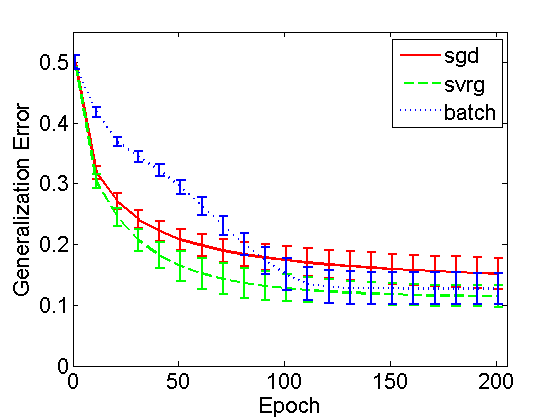
\includegraphics[scale=0.33]{Synthetic_GNMDS_200_test.png}
			}
			%\subfigure[CKL]
			%{
			%	\label{fig:1:subfig:b} %% label for second subfigure
			%	%\includegraphics[scale=0.24]{Synthetic_CKL_200_test_crop.png}
			%	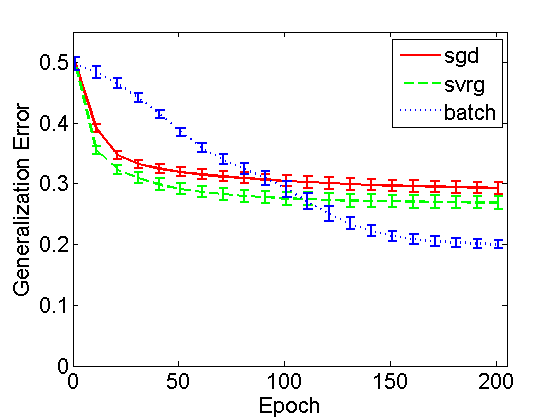
\includegraphics[scale=0.24]{Synthetic_CKL_200_test.png}
			%}
			%\vspace{0.5cm}
			\subfigure[STE]
			{
				\label{fig:1:subfig:c} %% label for third subfigure
				%\includegraphics[scale=0.24]{Synthetic_STE_200_test_crop.png}
				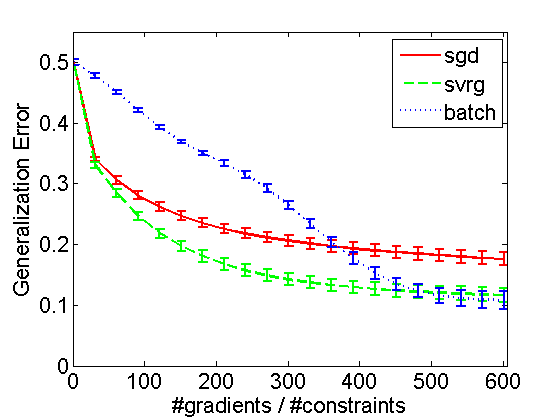
\includegraphics[scale=0.33]{Synthetic_STE_200_test.png}
			}
			\subfigure[TSTE]
			{
				\label{fig:1:subfig:d} %% label for fourth subfigure
				%\includegraphics[scale=0.24]{Synthetic_TSTE_200_test_crop.png}
				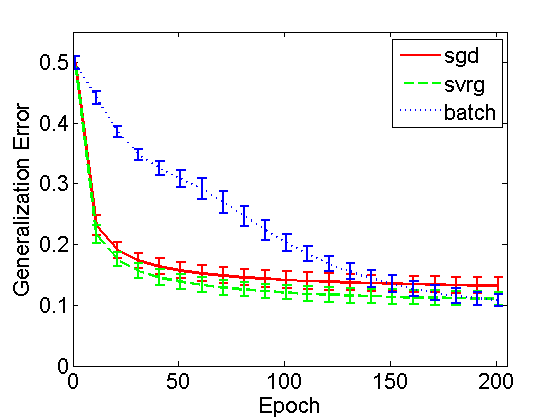
\includegraphics[scale=0.33]{Synthetic_TSTE_200_test.png}
			}
			\caption{Generalization error of different optimization methoods on the synthetic data}
			\label{fig:1} %% label for entire figure
		\end{figure*}

		\section{Experiments}
		In this section, three examples are exhibited with both simulated and real-world data to illustrate the validity of the analysis above and applications of the methodology proposed. The first example is with simulated data while the latter two exploit real-world datasets. In the following, we focus on a special case of quadruple comparisons as $i=l$ and $\{i,j,i,k\}\subset[n]^3$. During all the experiments, we adopt $(i,j,k)$ to indicate the ordinal constrain $d^2_{ij}(\mathbf{X})\leq d^2_{ik}(\mathbf{X})$. We evaluate the stochastic non-convex formulation of three different ordinal embedding objective functions. We set the baseline as these objective functions solved by batch gradient descent and denote the results as ``batch''. In other words, we will compare the SGD and SVRG solutions of these objective functions to the batch results in details in this section.

		\subsection{Simulated Study}
		\subsubsection{Settings.}
		First, we start with a small-scale synthetic experiment to show how the methods perform in an idealized setting, which provides sufficient ordinal information in noiseless case. This dataset consists of $200$ points $\{\mathbf{x}_i\}_{i=1}^{200}\subset\mathbb{R}^{10}$, where $\mathbf{x}_i\sim\mathcal{N}(\mathbf{0}, \frac{1}{20}\mathbf{I})$ and $\mathbf{I}\subset\mathbb{R}^{10\times 10}$ is the identity matrix. The possible similarity triple comparisons are generated based on the Euclidean distances between $\{\mathbf{x}_i\}$. As \cite{2016arXiv160607081J} has proved that the Gram matrix $\mathbf{G}$ can be recovered from $O(pn\log n)$ triplets, we randomly choose $|\mathcal{C}|=10000$ triplets as the training set and the rest as the testing set.

		The metric that we used in the evaluation of the performance of various algorithms is the \textbf{generalization error}. As the learned embedding $\mathbf{X}$ from partial triple comparisons set $\mathcal{C}\subset[n]^3$ should generalize to unknown triplets as triplets are obtained and the generalization can help to model comprehensive relationships among all objects, the percentage of held-out triplets which is satisfied in the embedding $\mathbf{X}$ is used as the main metric for evaluating the quality.

		\qqxu{qqxu: Please rewrite this Para. which splits learning rate setting as a separate Para.}We evaluate non-convex formulation of three objective functions (i.e. GNMDS, STE and TSTE) solved by gradient descent, SGD and SVRG.
		%To enable a fair comparison, we show the generalization error of three optimization method with same calculation of (sub)gradient.
		The SVRG method is terminated after maximum of 200 epochs or when the change in Frobenius norm of embedding $\mathbf{X}$ between iterations is less than $10^{-5}$. As SVRG performs $2m+|\mathcal{C}|$ times of (sub)gradient in each epoch, the batch and SGD solutions are evaluated when they use the same numbers of (sub)gradient as SVRG. We set $m=|C|$ in all experiments. The $x$-axis of each figure is computational cost measured by the number of gradient evaluations divided by the total number of triple-wise constraints $|\mathcal{C}|$. The experiment is performed with $10$ trials of different, random initial $\mathbf{X}_0$. The generalization error in the figures is the mean of $10$ trials. The error bar in the all graphs represents the range between one unit of standard deviation.

		\textbf{Remark. }Learning rate is a critical parameter in gradient method and we adopt different strategies for the three optimization method in experiments. The learning rate of batch gradient descent is adjusted with a adaptive mechanism as: when the objective function $f(\mathbf{X}_t)$ is larger than $f(\mathbf{X}_{t-1})$, the learning rate will be $\eta_t=1.01\eta_{t-1}$; when the objective function $f(\mathbf{X}_t)$ is smaller than $f(\mathbf{X}_{t-1})$, the learning rate will be $\eta_t=0.5\eta_{t-1}$. We decrease the learning rate $\eta_t$ of SGD by learning rate scheduling as: exponential decay $\eta_t = \eta_0 a^{\left \lfloor \frac{t}{|\mathcal{C}|} \right \rfloor}$ with parameters $\eta_0$ and $a$ to adjust, and t-inverse $\eta_t = \eta_0(1 + b\left \lfloor \frac{t}{|\mathcal{C}|} \right \rfloor)^{-1}$ with $\eta_0$ and $b$ to adjust. For SVRG, we utilize a fixed step size as suggested by the aforementioned analysis. The relatively large $\eta$ with SVRG will lead to faster convergence than that of SGD.

		\subsubsection{Results.}
		Figure \ref{fig:1} shows the experimental results of three objective functions. From these experimental results, we make the following comments. First, it can be seen from this figure that with the increase of gradient computations, the generalization error curve generally decreases. Moreover, we note that at the initial stage, both SGD and SVRG could outperform the batch optimization with smaller generalization error. Although this does not hurt the long term behavior eventually, those who care the initial iterations should be careful on this. Finally, it can be seen that the SVRG method is able to maintain competitive performances with the batch case in the long run because of its ``variance-reduction property". 

		%The Figure \ref{fig:1} shows that the SVRG solutions perform the similar result as the batch solutions. The experiment results demonstrate the stochastic methods make a rapid initial progress as they use a single gradient on each iteration and outperform the batch methods by a large margin in early epochs. The experiments also show the comparison of convergence rate between SGD and SVRG as SGD operates more iterations than SVRG when they calculate the same number of (sub)gradients. The SVRG method, which reduces the variance of SGD, can use the gradients more efficient than SGD , obtain a better solution and converge faster than SGD.

		%\begin{table}[ht]
		%	\centering
		%	\label{tab:1}
		%	\begin{tabular}{c||c c c c c }
		%		\hline
		%				& Min 	 & Mean 	& Median 	& Max 		& SD 	    \\ \hline \hline \\
		%		SGD 	& 1.4440 & 1.6514 	& 1.6720 	& 1.8590 	& 0.1463    \\	\\ \hline    \\
		%		SVRG 	& 2.7040 & 2.9156 	& 2.9240 	& 3.3400 	& 0.2092 	\\  \\ \hline    \\
		%		Batch 	& 3.6730 & 4.2903 	& 4.2570 	& 5.6370 	& 0.5626	\\  \\ \hline
		%	\end{tabular}
		%	\caption{Run time (seconds) of GNMDS with different optimization methods on the synthetic data}
		%\end{table}
		\begin{table}[ht]
			\centering
			\begin{tabular}{c||c c c c c }
				\hline
						& Min 	 & Mean  	& Max 		& SD 	    \\ \hline \hline
				SGD 	& 1.4440 & 1.6514 	& 1.8590 	& 0.1463    \\ \hline
				SVRG 	& 2.7040 & 2.9156 	& 3.3400 	& 0.2092 	\\   \hline
				Batch 	& 3.6730 & 4.2903 	& 5.6370 	& 0.5626	\\   \hline
			\end{tabular}
			\caption{Run time (seconds) of GNMDS with different optimization methods on the synthetic data}\label{tabl1}
		\end{table}
		%\begin{table}[ht]
		%	\centering
		%	\label{tab:2}
		%	\begin{tabular}{c||c c c c c }
		%		\hline
		%				& Min 	 & Mean 	& Median 	& Max 		& SD 		\\ \hline \hline    \\
		%		SGD 	& 2.7730 & 3.4780 	& 3.3825 	& 4.3540 	& 0.5368 	\\ \\ \hline        \\
		%		SVRG 	& 3.9320 & 4.4594 	& 4.4420 	& 4.9810 	& 0.3978 	\\ \\ \hline        \\
		%		Batch 	& 5.9070 & 6.9870 	& 6.8095 	& 8.2420 	& 0.8785 	\\ \\ \hline
		%	\end{tabular}
		%	\caption{Run time (seconds) of STE with different optimization methods on the synthetic data}
		%\end{table}
		\begin{table}[ht]
			\centering
			\begin{tabular}{c||c c c c c }
				\hline
						& Min 	 & Mean 	& Max 		& SD 		\\ \hline \hline
				SGD 	& 2.7730 & 3.4780 	& 4.3540 	& 0.5368 	\\  \hline
				SVRG 	& 3.9320 & 4.4594 	& 4.9810 	& 0.3978 	\\  \hline
				Batch 	& 5.9070 & 6.9870 	& 8.2420 	& 0.8785 	\\  \hline
			\end{tabular}
			\caption{Run time (seconds) of STE with different optimization methods on the synthetic data}\label{tab_2}
		\end{table}
		%\begin{table}[ht]
		%	\centering
		%	\label{tab:3}
		%	\begin{tabular}{c||c c c c c }
		%		\hline
		%				& Min 	 & Mean 	& Median 	& Max 		& SD 		\\ \hline \hline \\
		%		SGD 	& 4.1470 & 6.9635 	& 7.1015 	& 9.8380 	& 2.1108 	\\ \\   \hline   \\
		%		SVRG 	& 4.6610 & 5.6840 	& 5.4085 	& 7.5680 	& 1.0041 	\\ \\   \hline   \\
		%		Batch 	& 9.3940 & 10.4511 	& 10.0830 	& 13.4060 	& 1.2199 	\\ \\   \hline
		%	\end{tabular}
		%	\caption{Run time (seconds) of TSTE with different optimization methods on the synthetic data}
		%\end{table}
		\begin{table}[ht]
			\centering
			\begin{tabular}{c||c c c c c }
				\hline
						& Min 	 & Mean 	& Max 		& SD 		\\ \hline \hline
				SGD 	& 4.1470 & 6.9635 	& 9.8380 	& 2.1108 	\\    \hline
				SVRG 	& 4.6610 & 5.6840 	& 7.5680 	& 1.0041 	\\    \hline
				Batch 	& 9.3940 & 10.4511 	& 13.4060 	& 1.2199 	\\    \hline
			\end{tabular}
			\caption{{Run time (seconds) of TSTE with different optimization methods on the synthetic data}}\label{tab_3}
		\end{table}

		The results of practical run time are exhibited in Table \ref{tabl1}-\ref{tab_3}. We record the time of the three objective functions solved by batch gradient descrnt, SGD and SVRG before the training error is larger than $0.1$ in $10$ trials. All objective functions optimized by SVRG and SGD gains speeded-up compared to the batch case. Although SGD is a bit faster than SVRG and batch, the generalization of the SGD embedding is inferior to the SVRG embedding. The low standard deviation of SVRG indicates that the acceleration is statistical stable. GNMDS use the hinge loss which is a truncated function and only assigns a penalty to violated ordinal constraint $(i,j,k)$, and STE $\&$ TSTE not only penalize the violations but also provide reward for the embedding $\{\mathbf{x}_i, \mathbf{x}_j, \mathbf{x}_k\}$ which are satisfied the ordinal constraint $(i,j,k)$. The pratical run time of GNMDS is less than that of STE and TSTE. TSTE employs heavy-tailed similarity kernel to compute triplet probabilities from an embedding rather than the Gaussian kernel in STE, and needs more time to show the same train error compared to the STE.
		
		\begin{figure*}
			\centering
			\subfigure[GNMDS]
			{
				\label{fig:2:subfig:a} %% label for first subfigure
				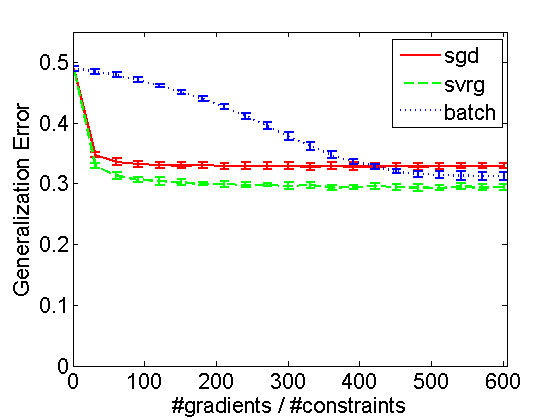
\includegraphics[scale=0.33]{MNIST_GNMDS_200_test.png}
			}
			%\subfigure[CKL]
			%{
			%	\label{fig:2:subfig:b} %% label for second subfigure
			%	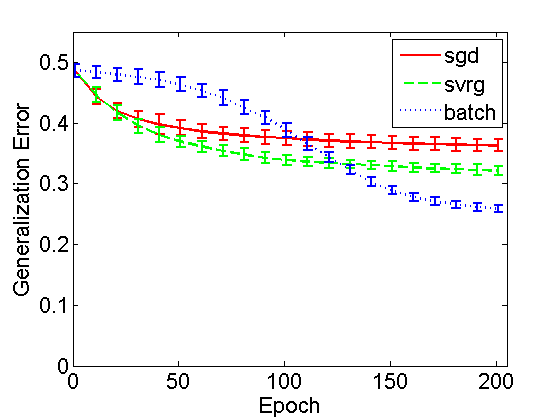
\includegraphics[scale=0.24]{MNIST_CKL_200_test.png}
			%}
			%%\vspace{0.5cm}
			\subfigure[STE]
			{
				\label{fig:2:subfig:c} %% label for first subfigure
				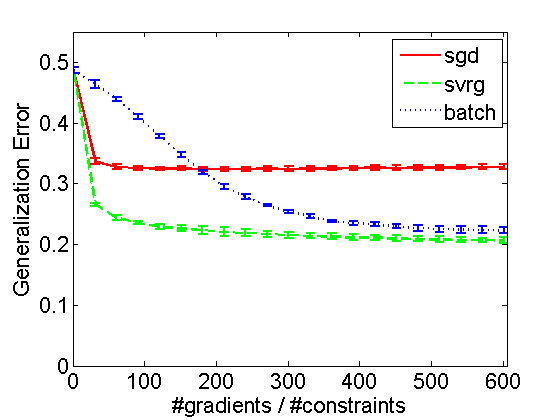
\includegraphics[scale=0.33]{MNIST_STE_200_test.png}
			}
			\subfigure[TSTE]
			{
				\label{fig:2:subfig:d} %% label for second subfigure
				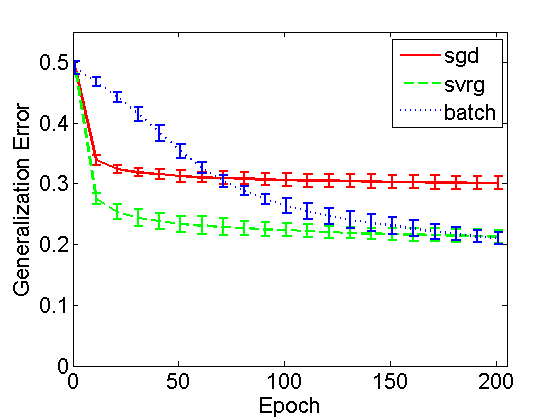
\includegraphics[scale=0.33]{MNIST_TSTE_200_test.png}
			}
			\caption{Generalization error of SGD, SVRG and batch optimization on the MNIST data}
			\label{fig:2} %% label for entire figure
		\end{figure*}
		\begin{figure*}
			\centering
			\subfigure[GNMDS]
			{
				\label{fig:3:subfig:a} %% label for first subfigure
				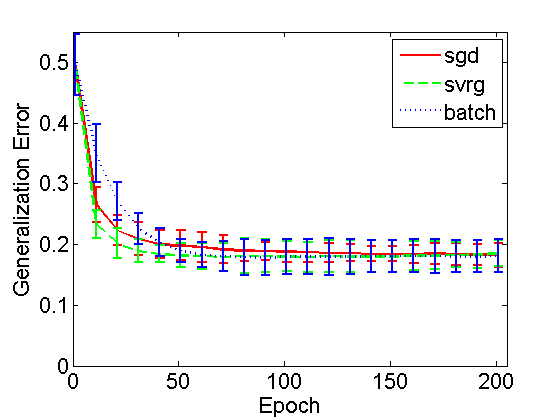
\includegraphics[scale=0.33]{Music_GNMDS_200_test.png}
			}
			%\subfigure[CKL]
			%{
			%	\label{fig:3:subfig:b} %% label for second subfigure
			%	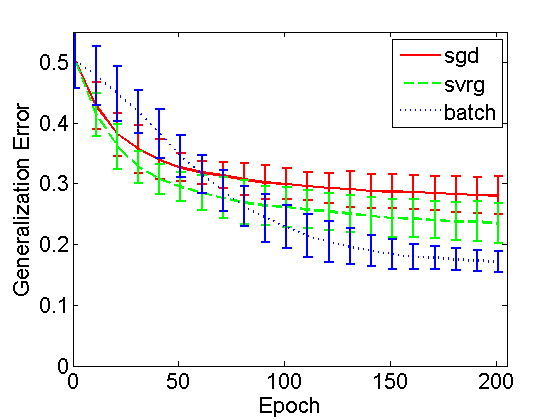
\includegraphics[scale=0.24]{Music_CKL_200_test.png}
			%}
			%\vspace{0.5cm}
			\subfigure[STE]
			{
				\label{fig:3:subfig:c} %% label for first subfigure
				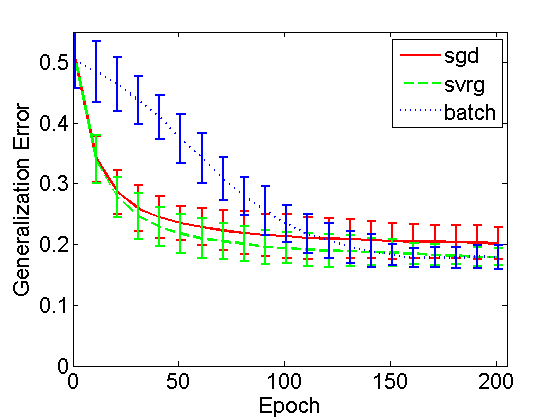
\includegraphics[scale=0.33]{Music_STE_200_test.png}
			}
			\subfigure[TSTE]
			{
				\label{fig:3:subfig:d} %% label for second subfigure
				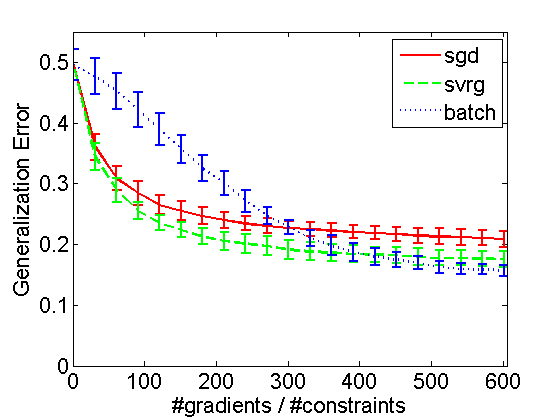
\includegraphics[scale=0.33]{Music_TSTE_200_test.png}
			}
			\caption{Generalization error of SGD, SVRG and batch optimization on the music artist data}
			\label{fig:3} %% label for entire figure
		\end{figure*}

		\subsection{MNIST Handwriting Data}
		\subsubsection{Settings.}
		The experiment on MNIST follows the settings like \cite{vandermaaten2012stochastic}. We randomly select a subset of $n=1000$ digits from the MNIST data set, and the similarity triple comparisons are generated by the Euclidean distances between the $784$ dimension raw pixel vectors. As the complete set of triplets are cumbersome for handling, we randomly sample $100000$ triplets for training and testing. For each $(i, j, k)$, $i$ is picked uniformly at random, $j$ is uniformly chosen among the $50$ nearest neighbors of $i$, and $k$ is uniformly chosen from the set of digits that are further away from $i$ than $j$. The digit labels are not used in the procedure and the generation introduces noisy comparisons into the triplets. For each trial of the data set, we randomly pick $90000$ triplets as the train set and the rest would be the test set. This data set focus on the performance of these methods with noisee ordinal information. The desired dimension of embedding is $p = 10$ as digits fall into $10$ categories. The results of different embedding dimensions can be found in supplementary.
		\subsubsection{Results.}
		The experiment results of MNIST data set are illustrated in Figure \ref{fig:2:subfig:a}-\ref{fig:2:subfig:d}. The SVRG reduces the variance and  converges faster than the batch method in the three cases of differernt objective function. The generalization of SGD embedding is worse than that of SVRG and batch embedding. We conjecture that the noise ordinal constraints will damege the generalization of the embedding and the variance of SGD exacerbate the the problem. The experiment on this data set demonstrate the variance reduction is an essential issue in embedding problem when we employ stochastic optimization.

		\subsection{Music Artist Data}
		\subsubsection{Settings.}
		The music artist data is collected by \cite{ellis2002quest} via a web-based survey in which $1032$ users provided $213472$ triplets on the similarity of $412$ music artists. We use the data pre-processed by \cite{vandermaaten2012stochastic} and only $9107$ triplets for $n=400$ artists remain. For each trial of the data set, the $90\%$ triplets are randomly picked as the train set and the rest comparisons are used are the test set. This data set focus on the result of these methods with a small quantity of ordinal information. The desired dimension of embedding is $p = 9$ as these music artists can be classified by their genres into $9$ categories. We provide other embedding results with different dimensions in supplementary.
		\subsubsection{Results.}
		Although the train set of this experiment only provide little ordinal information, the SVRG optimization can still outperform both SGD and batch method. Under these settings, the gap between the SVRG and SGD method is small. The stochastic methods, especially the SVRG, are still more efficient than batch method.

		%In this section, we present the empirical results. As the number of quadruple comparisons as $\{(i,j,l,k)\}\subset[n]^4$ is tremendous and there are few real-world data sets provide such ordinal information, we focus the special case of quadruple comparisons as $i=l$ and $\{i,j,i,k\}\subset[n]^3$. During all experiments, we \qqxu{adopt} $(i,j,k)$ to indicate the ordinal constrain $d^2_{ij}(\mathbf{X})\leq d^2_{ik}(\mathbf{X})$. \qqxu{Before illustrating the experimental results, we firstly explain why we choose batch solution of (\ref{eq:2}) as the baseline.}

		%\subsection{Baseline Selection}
		%We discuss the performance gap between the convex and non-convex solutions for embedding problem. For practical applications,  As the desired dimension $p$ is given, we need to tune the regularization parameter $\lambda$ of (\ref{eq:1}) to obtain a $\mathbf{G}$ with $\text{rank}(\mathbf{G})=p$ and keep the intermediate results $\{\mathbf{G}_t\}$ being low-rank. This requirement is not trivial in practical applications as the high computational cost of SDP and SVD. Without low-rank Gram matrix $\mathbf{G}$, the embedding $\mathbf{X}$ from convex formulation (\ref{eq:1}) will be worse than non-convex formulation (\ref{eq:2}) (need more analysis). We show the performance gap between the two formulations in supplementary and the gap always exists in all our experiments. So non-convex formulation (\ref{eq:2}) with batch gradient descent is chosen as the baseline for further comparison.
		
		%\subsection{Experimental Setup}
		%We evaluate batch, SGD and SVRG versions of GNMDS, STE and TSTE on three different data sets, each with its own challenges for ordinal embedding problem.  Second, a data set of similarity triple comparisons over popular music artists \cite{ellis2002quest} is used to evaluate how the methods perform in a real-world setting with moderate triplet noise. Finally, all methods are evaluated on a data set of triplets over MNIST, which consist of a small proportion of possible similarity triple comparisons, thus focusing on the performance of these methods with very little feedback. The experiments are performed with the following specifications unless otherwise noted. The batch GNMDS, STE and TSTE implementations specified by \cite{vandermaaten2012stochastic}. The SGD and SVRG optimization for each method are implemented by MATLAB with mex function.

		%\subsection{Synthetic Data}
		%The first experiment is to test all methods on an ideal, small-scale, synthetic data set. This data set consist of $200$ points $\{\mathbf{x}_i\}_{i=1}^{200}\subset\mathbb{R}^{10}$, where $\mathbf{x}_i\sim\mathcal{N}(\mathbf{0}, \frac{1}{20}\mathbf{I}_{10})$ and $\mathbf{I}_{10}\subset\mathbb{R}^{10\times 10}$ is the identity matrix. The possible similarity triple comparisons are generated based on the Euclidean distances between $\{\mathbf{x}_i\}$. As \cite{2016arXiv160607081J} has proved that the Gram matrix $\mathbf{G}$ can be accurately recovered from $O(pn\log n)$ triplets, we randomly choose $|\mathcal{C}|=10000$ triplets as the train set and the rest are used as the test set.
		
		%\subsection{MNIST Handwriting Data}
		
		%\subsection{Music Artist Data}

		\section{Conclusion and Future Work}

		In this paper, we propose a framework to learn representation from relative similarity comparisons by stochastic non-convex ordinal embedding. By taking advantage of the sparse structure of the gradients, we show how to operate stochastic gradient descent updates and analyze the non-asymptotic convergence. Further, we show how variance reduction benefits non-convex ordinal embedding in terms of accelerating the local convergence rate of SGD. Experimentally, we show on synthetic and real-world data that the proposed method converges much faster than the batch gradient descent method. With variance reduction, the stochastic optimization generalize well on held-out relative similarity comparisons and give the comparable performance. For future work, % wish to improve ordinal embedding in the following ways. First, we will explore a convex formulation for directly optimize the embedding $\mathbf{X}$. Second, we will investigate novel optimization for obtaining the uniqueness solution as some theoretical works have stated its existence \cite{2015arXiv150102861A,53e99af7b7602d97023851bf}. Finally, 
		we will strengthen the ordinal embedding algorithm by explicitly handling the noise ordinal constraints as they are always observed in real-world data. This can be done out of model using a robust ranking methods \cite{2014arXiv1408.3467X}.

		\bibliographystyle{aaai}
		\bibliography{aaai_17_svrg_ordinal_embedding}

	\end{document}
